\section{Decodificación de stream de datos en Simulink}

Como una primera comprobación del funcionamiento del sistema diseñado en Simulink se aprovechó la utilidad que tiene el prototipo de adquisición de enviar señales test (ondas cuadradas con frecuencia de 2 Hz). Se configuraron los 8 canales del prototipo de adquisición para que enviaran dicha señal test, cada uno con una ganancia diferente. Posteriormente se realizó un registro de forma continua en el que se visualizó en un scope el resultado del sistema decodificador. Adicional a esto, se realizaron registros de sEMG de un solo canal mientras se realizaba la tarea de cierre de mano. En la Figura \ref{Figura: Test_PADQ} se muestra el resultado de la adquisición de las señales test, mientras que en la Figura \ref{Figura: sEMG_PADQ} se muestra el resultado de un registro de sEMG. Ambos registros se realizaron configurando el prototipo de adquisición a una frecuencia de muestreo de 1 kHz.

\begin{figure}[htbp]
	\centering
	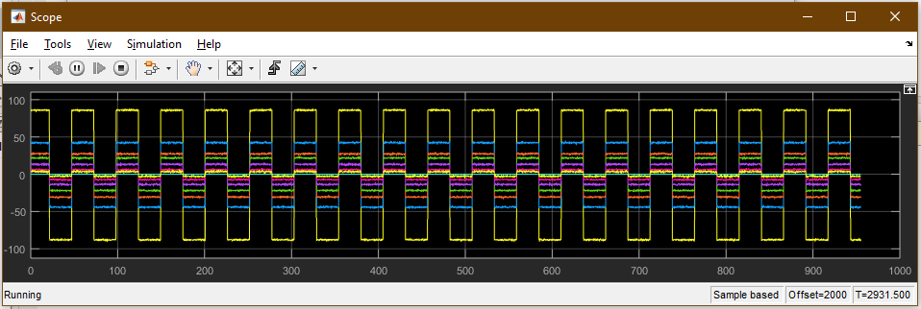
\includegraphics[width=0.8\textwidth]{Test_8CHs_1k_mue2mue.png}
	\caption{Resultado de la adquisición de los 8 canales del prototipo de adquisición configurado con señales test a diferentes ganancias.}
	\label{Figura: Test_PADQ}
\end{figure}

\begin{figure}[htbp]
	\centering
	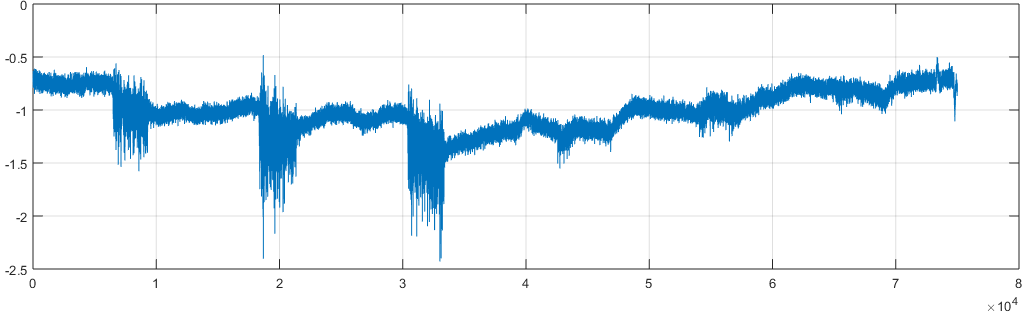
\includegraphics[width=0.8\textwidth]{sEMG_PADQ.png}
	\caption{Registro de sEMG de un solo canal a una frecuencia de muestreo de 1 kHz.}
	\label{Figura: sEMG_PADQ}
\end{figure}

\section{Evaluación de transferencia de datos entre prototipo de adquisición y computadora}

Adicional al procedimiento realizado para la evaluación de la comunicación, se realizó una medición de la frecuencia de muestreo real del sistema, esto se realizó midiendo con un osciloscopio la frecuencia con la que se activa el pin DRDY del ADS1299 (la activación de este pin indica que se ha realizado la adquisición de una muestra). El resultado de esta medición arrojó como resultado que la frecuencia de muestreo real del prototipo de adquisición es de 964.3 Hz. En la Figura \ref{Figura: DRDY} se muestra una captura de pantalla de la medición realizada.

\begin{figure}[htbp]
	\centering
	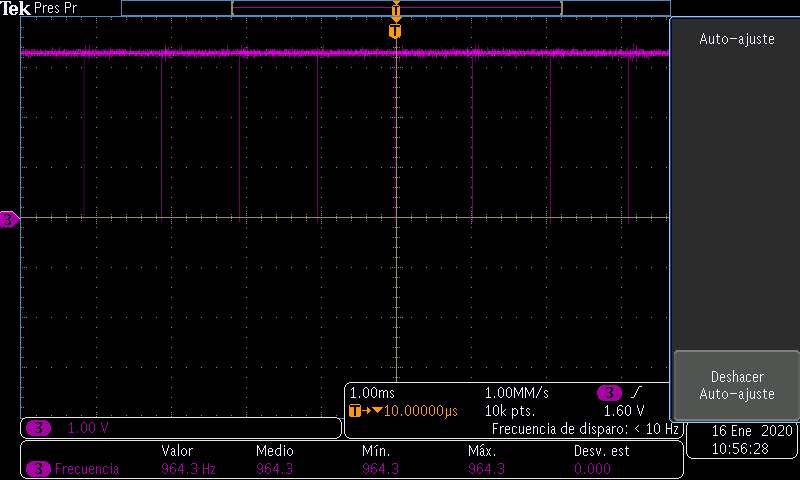
\includegraphics[width=\textwidth]{DRDY.png}
	\caption{Resultado de la medición de la frecuencia de muestreo real del prototipo de adquisición.}
	\label{Figura: DRDY}
\end{figure}

Posterior a esto se realizó un ajuste a la frecuencia de muestreo a las señales sintéticas en MATLAB, esto para que la frecuencia de muestreo sintética coincidiera con la frecuencia de muestreo real del prototipo de adquisición. Teniendo las señales sintéticas ajustadas a la nueva frecuencia de muestreo se procedió a calcular la correlación entre la señal sintética y la señal adquirida con el prototipo de adquisición. Una vez obtenidos todos los valores de correlación se calculó el promedio de estos, obteniendo como resultado una correlación promedio de 0.9615. En el Cuadro \ref{Cuadro: Corre} se muestran los resultados de la correlación obtenida para cada registro realizado.

\begin{table}[htbp]
\centering
\begin{tabular}{|c|c|c|c|}
\hline
\textbf{Señal}                                                   & \textbf{Registro 1} & \textbf{Registro 2} & \textbf{Registro 3} \\ \hline
Sen 1 Hz                                                         & 0.9868              & 0.9899              & 0.9899              \\ \hline
Sen 5 Hz                                                         & 0.8554              & 0.9750              & 0.9980              \\ \hline
Sen 10 Hz                                                        & 0.9985              & 0.9946              & 0.9912              \\ \hline
Sen 20 Hz                                                        & 0.9923              & 0.9930              & 0.9947              \\ \hline
Sen 50 Hz                                                        & 0.9828              & 0.9732              & 0.9851              \\ \hline
Sen 100 Hz                                                       & 0.9320              & 0.9309              & 0.9374              \\ \hline
\begin{tabular}[c]{@{}c@{}}Atenuación\\ lineal\end{tabular}      & 0.9677              & 0.9851              & 0.8869              \\ \hline
\begin{tabular}[c]{@{}c@{}}Atenuación\\ exponencial\end{tabular} & 0.7149              & 0.9523              & 0.9874              \\ \hline
Contracción                                                      & 0.9877              & 0.9896              & 0.9916              \\ \hline
\end{tabular}
\caption{Resultados de la correlación obtenida entre las señales sintéticas y los registros realizados con el prototipo de adquisición.}
\label{Cuadro: Corre}
\end{table}

\section{Procesamiento de sEMG}

Optando por utilizar como descriptor de la amplitud del sEMG al valor RMS se procedió a realizar pruebas sobre el desempeño de este. Se realizaron registros de sEMG filtrados con el filtro pasa altas descrito en la metodología y utilizando ventanas de registro de 100 mS, estas ventas de registro se utilizaron para calcular el valor RMS de ellas y dicho valor se visualizó en un scope en Simulink. En la Figura \ref{Figura: RMS_Filter} se muestra un segmento de uno de los registros realizados en esta prueba.

\begin{figure}[htbp]
	\centering
	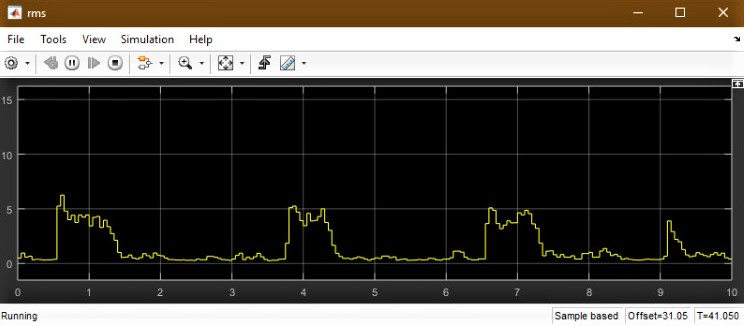
\includegraphics[width=\textwidth]{RMS_Filter_2.png}
	\caption{Resultado del cálculo del valor RMS utilizando ventanas de registro con duración de 100 mS mientras se realizaba la tarea de cierre de mano.}
	\label{Figura: RMS_Filter}
\end{figure}

\newpage
\section{Mapeo sEMG-FES}
Como una primera prueba de la utilidad de una transformación lineal como mapeo de sEMG a FES se utilizó un generador de funciones para generar una senoidal de  20 Hz e ir variando su amplitud de tal forma que simulara variaciones en la amplitud del sEMG. Se utilizó como parámetros de la recta los siguientes: $A_{min}=0[A]$, $A_{max}=50[A]$, $D_{min}=60$, $D_{max}=1500$. Dichos parámetros se configuraron en un bloque \emph{Fcn} de Simulink en la forma descrita por la Ecuación \ref{Mapeo} (Sección 4.5). Para visualizar los efectos de aplicar este mapeo al valor RMS se visualizó en dos scopes los valores obtenidos de RMS y los resultantes tras aplicar el mapeo. En la Figura \ref{Figura: Map1_Sen} se muestra el resultado de ambos valores al ir variando la amplitud de la senoidal generada por el generador de funciones.

\begin{figure}
	\centering
	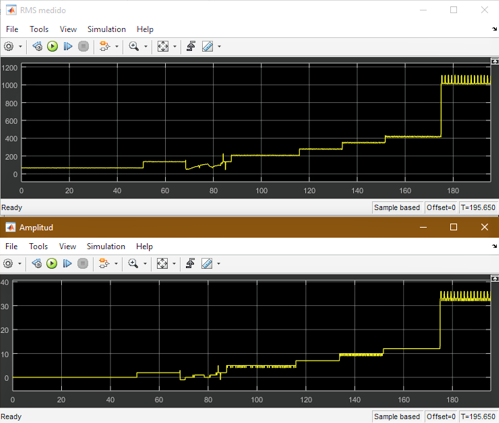
\includegraphics[width=\textwidth]{Mapeo1_Seno.png}
	\caption{Resultados de valor RMS (arriba) y mapeo (abajo) al ir variando la amplitud de una senoidal de 20 Hz.}
	\label{Figura: Map1_Sen}
\end{figure}
